\documentclass[unknownkeysallowed]{beamer}
\usepackage{minted}
\usepackage{beamerthemeWuppertal}
\usepackage[utf8]{inputenc}
\usepackage{german}

\title{Eine Anwendung zur Darstellung verschiedener Fraktale mit Qt 5}
\author{Dimitri Tarnavski}
\date{18. Mai 2017}

\begin{document}
\maketitle

\tableofcontents[hideallsubsections]


% Erster Abschnitt, Klären des Begriffs "Fraktal"
\section{Was ist ein Fraktal}

\subsection{Definition des Begriffs}

\begin{frame}
  \frametitle{Was ist ein Fraktal?}
  \begin{itemize}
    \item 1975 vom Mathematiker Benoît Mandelbrot geprägt
    \item Aus dem lat. \emph{fractus} "`gebrochen"', "`in Teile gebrochen"'
    \item Bezeichnet bestimmte \emph{selbstähnliche} Muster/Strukturen
  \end{itemize}
\end{frame}

\subsection{Selbstähnlichkeit}

\begin{frame}
  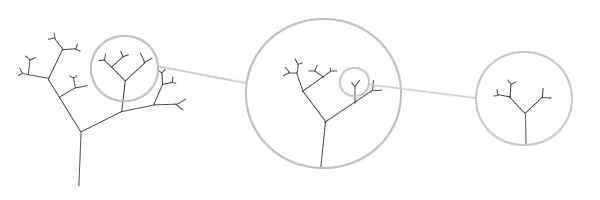
\includegraphics[width=1\textwidth]{images/fractal1.jpg}
  \begin{itemize}
    \item Keine perfekte Kopie des Baums
    \item Eine Linie ist selbstähnlich, jedoch kein Fraktal
  \end{itemize}
\end{frame}

\subsection{Fraktale in der Natur}
\begin{frame}
  Fraktale Strukturen können oft in der Natur beobachtet werden:
  \begin{itemize}
    \item Bäume
    \item Blitze
    \item Berge und Küsten
    \item Blutgefäße
  \end{itemize}
  \vspace{5mm} %5mm vertical space
  Eine fraktale Struktur ist immer mit rekursivem Verhalten verbunden.
\end{frame}


\section{Drei konkrete Fraktale}

\subsection{Kochschneeflocke}
\begin{frame}
  \frametitle{Die Kochschneeflocke}
  \begin{figure}[ht]
    \centering
    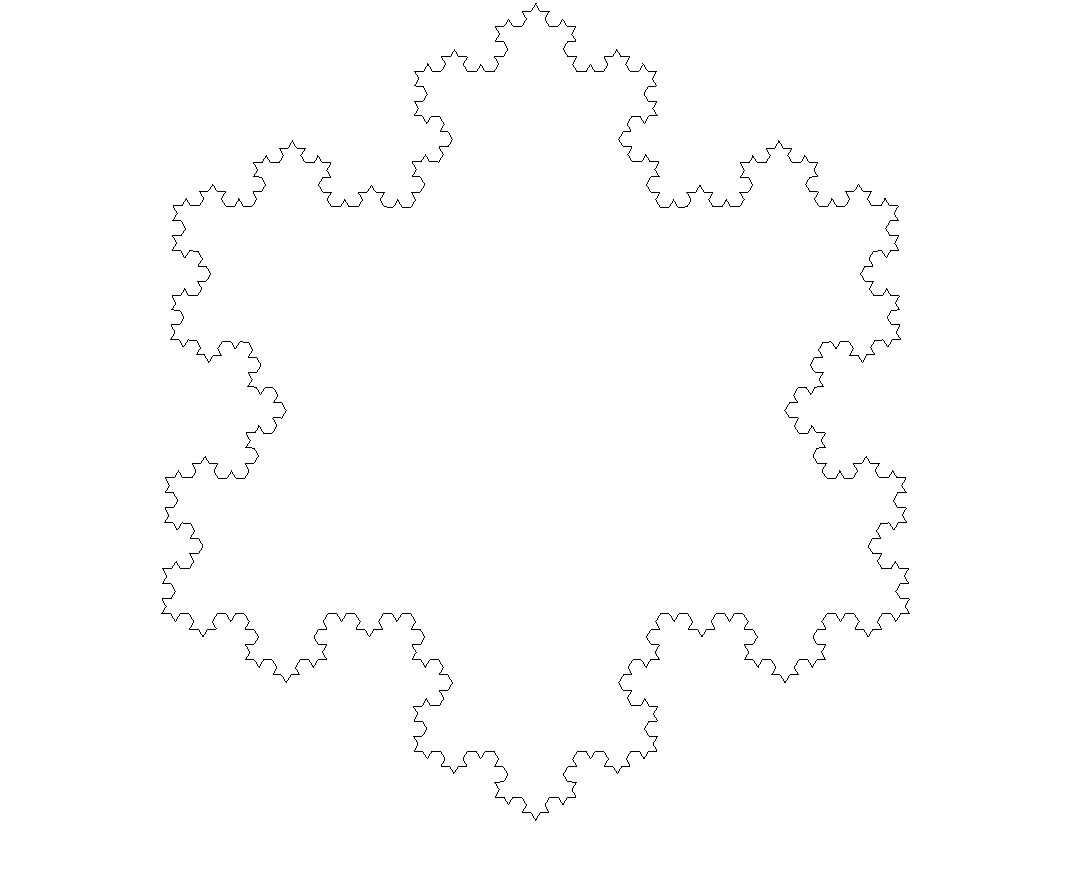
\includegraphics[width=0.8\textwidth]{images/fractal-koch.png}
  \end{figure}
\end{frame}

\begin{frame}
  \frametitle{Konstruktion der Kochlinie}
  \begin{figure}[ht]
    \centering
    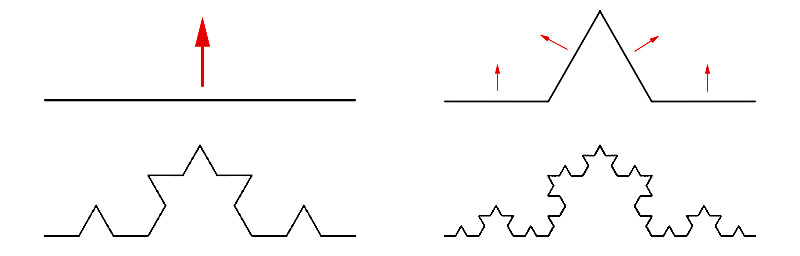
\includegraphics[width=0.8\textwidth]{images/how-to-koch.jpg}
    \caption{Konstruktion der Koch-Kurve, Quelle: Wikipedia}
  \end{figure}
\end{frame}

\begin{frame}[fragile]
  \frametitle{Berechnen der einzelnen Punkte}
  \begin{minipage}{0.5\textwidth}
  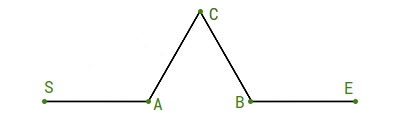
\includegraphics[width=\textwidth]{images/how-to-koch-2.jpg}
  \end{minipage}
  \begin{minipage}{0.48\textwidth}
    S = Anfangspunkt der Linie\\
    E = Endpunkt der Linie\\
    Diff = Differenz zwischen S \& E
  \end{minipage}

  \begin{minted}{c++}
  A.x = S.x() + Diff.x() / 3.0;
  A.y = S.y() - Diff.y() / 3.0;

  B.x = S.x() + 2.0 * Diff.x() / 3.0;
  B.y = S.y() - 2.0 * Diff.y() / 3.0;

  C.x = S.x() + Diff.x() / 2.0 - H * Diff.y() / 1.4;
  C.y = S.y() - Diff.y() / 2.0 - H * Diff.x();
  \end{minted}
\end{frame}

\subsection{Mandelbrot-Menge}
\begin{frame}
  \frametitle{Die Mandelbrot-Menge}
  \begin{figure}[ht]
    \centering
    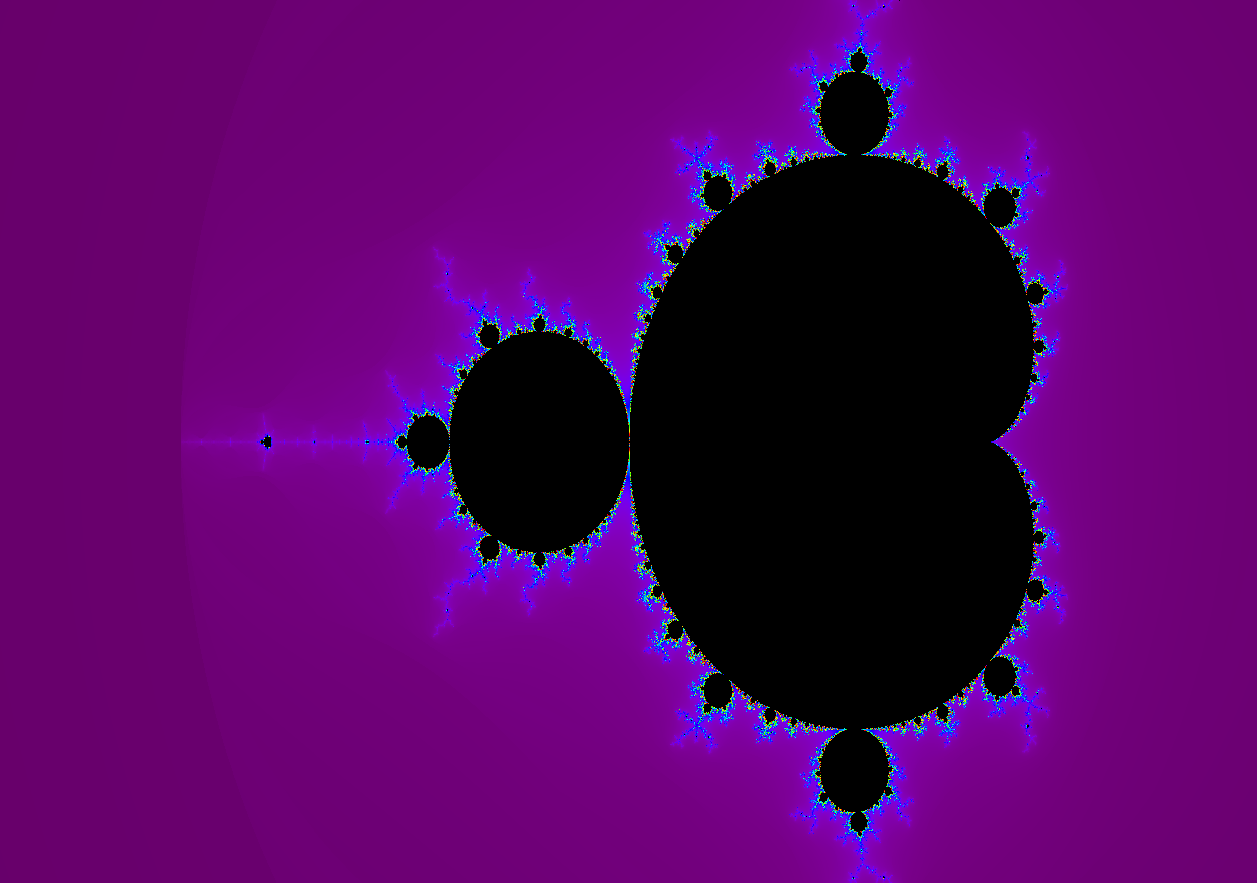
\includegraphics[width=0.8\textwidth]{images/fractal-mandelbrot.png}
  \end{figure}
\end{frame}

\begin{frame}
  \frametitle{Definition der Menge}
  Die Mandelbrot-Menge wird definiert durch die rekursiv definierte Folge:
  \begin{equation*}
    z_{n+1} = z^2_n + c, z_0 = 0, c \in \mathbb{C}
  \end{equation*}
  Zerlegt in Realteil und Imaginärteil:
  \begin{equation*}
    x_{n+1} = x^2_n - y^2_n + c_x
  \end{equation*}
  \begin{equation*}
    y_{n+1} = 2 \cdot x_n \cdot y_n + c_y
  \end{equation*}
\end{frame}

\begin{frame}[fragile]
  \begin{minted}{c++}
    for Alle Pixel (pX, pY):
      double x0 = pX abgebildet in [-2, 1]
      double y0 = pY abgebildet in [-1, 1]
      double x, y, iterations = 0;
      while(
        x * x + y * y < 4 && iterations < maxIterations
      ) {
        double xtemp = x * x - y * y + x0;
        y = 2 * x * y + y0;
        x = xtemp;
        iterations++;
      }
  \end{minted}
\end{frame}

\subsection{Julia-Menge}
\begin{frame}
  \frametitle{Die Julia-Menge}
  \begin{figure}[ht]
    \centering
    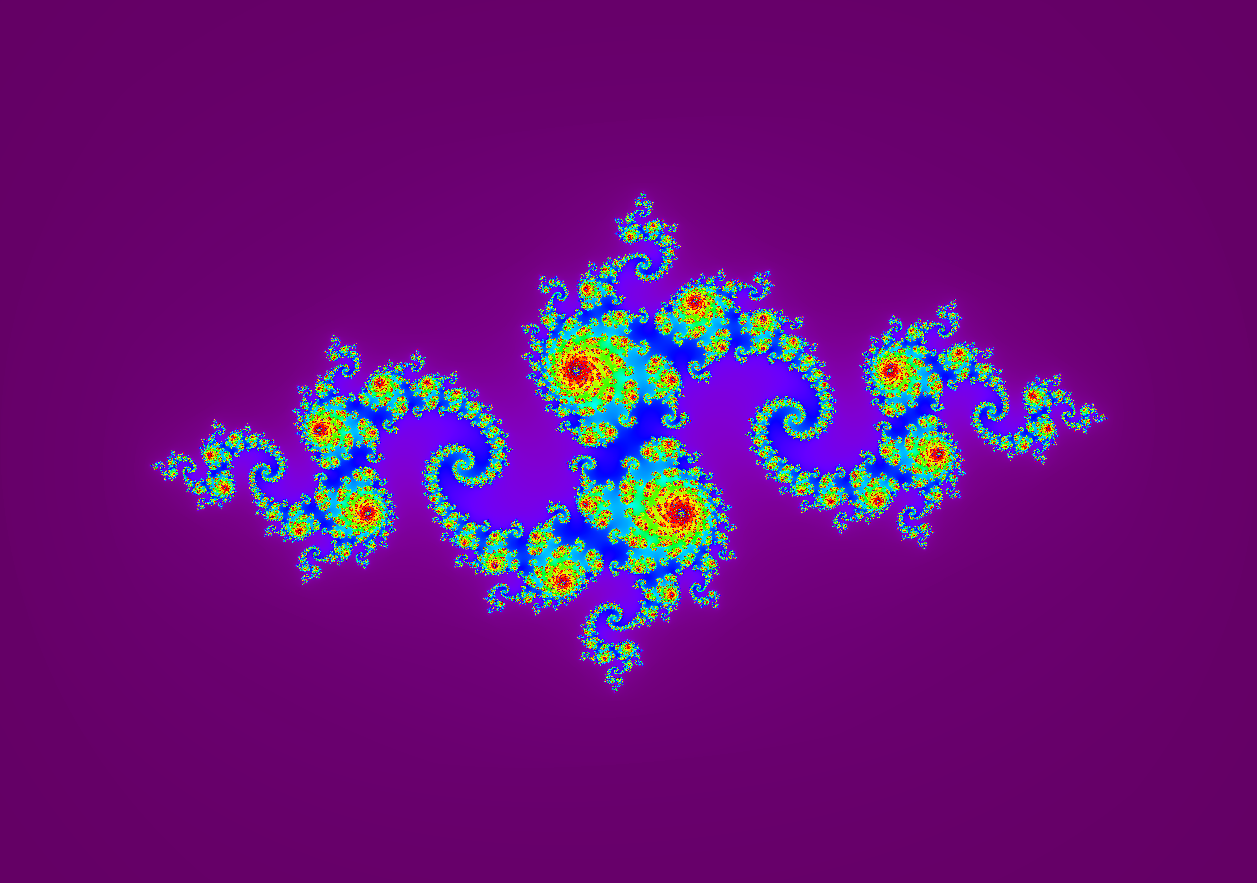
\includegraphics[width=0.8\textwidth]{images/fractal-julia.png}
  \end{figure}
\end{frame}

\begin{frame}
  Definiert wie die Mandelbrot-Menge für ein festes c.
  \begin{equation*}
    z_{n+1} = z^2_n + c, z_0 = 0, c \in \mathbb{C} fixiert
  \end{equation*}
  \begin{itemize}
    \item Es gibt viele Julia-Mengen.
  \end{itemize}
\end{frame}

\begin{frame}
  \begin{figure}[ht]
    \centering
    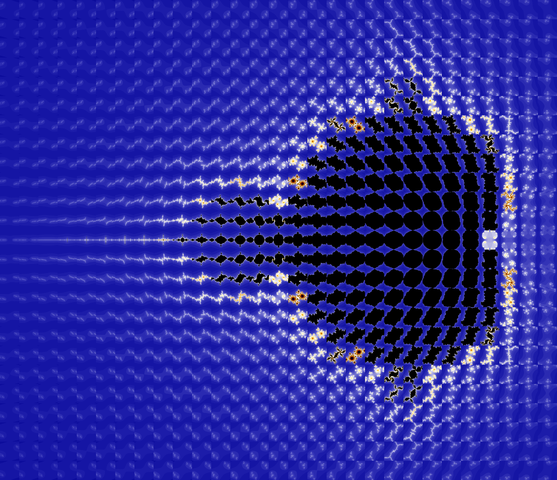
\includegraphics[width=0.7\textwidth]{images/julia-sets.png}
    \caption{Julia-Mengen für verschiedene c, Quelle: Wikipedia}
  \end{figure}
\end{frame}


\section{Implementierung}

\subsection{Klassendiagramm}

\begin{frame}
  \frametitle{Das Klassendiagramm}
  Es gibt drei wichtige Klassen:
  \begin{itemize}
    \item Fractal - Elternklasse für alle Fraktale
    \item RenderTask - Elternklasse für Rendering-Aufgaben
    \item ColorMode - Elternklasse für Farbgebunden
  \end{itemize}
\end{frame}

\subsection{Das Hauptfenster}

\begin{frame}
  \begin{itemize}
    \frametitle{Das Hauptfenster}
    \item Nimmt Benutzereingaben entgegen
    \item Ruft entsprechende Funktionen des aktuellen Fraktals auf
    \begin{itemize}
      \item Z.B. Skalieren und Verschieben
    \end{itemize}
    \item Stellt Funktionen zum Im-/Exportieren eines Fraktals
  \end{itemize}
\end{frame}

\begin{frame}[fragile]
  \frametitle{Hinzufügen eines Fraktals}
  \begin{minted}{c++}
  // Registriere die Fraktale, welche in der
  // Applikation ausgewählt werden können.
  registerFractal<EmptyFractal>(
    Fractals::ID::EMPTY_FRACTAL, "Keine Auswahl"
  );
  registerFractal<Mandelbrot>(
    Fractals::ID::MANDELBROT, "Mandelbrot-Menge"
  );
  ...
  \end{minted}
\end{frame}

\begin{frame}[fragile]
  \begin{minted}[fontsize=\footnotesize]{c++}
  std::map<
    Fractals::ID, std::function<Fractal::Ptr()>
  > fractalFactory;
  ...
  template<typename T>
  void FractalWindow::registerFractal(
    Fractals::ID fractalID, QString label
  ) {
    // Fügt einen Eintrag zu der Combobox der Fraktale hinzu.
    fractalsCombo->addItem(label, QVariant::fromValue(fractalID));
    // Speichert eine Funktion zum Erzeugen eines neuen Fraktals,
    // welche bei Bedarf durch Ausführen ein neues Fraktal generiert.
    fractalFactory[fractalID] = [this] () -> Fractal::Ptr {
      return Fractal::Ptr(new T(
        canvas.size().width(), canvas.size().height()
      ));
    };
  }
  \end{minted}
\end{frame}

\subsection{Die Klasse Fractal}
\begin{frame}[fragile]
  \frametitle{Reaktivität der Einstellungen}
  \begin{minted}[fontsize=\footnotesize]{c++}
  QSpinBox* iter = new QSpinBox;
  ...
  connect(
    iter, static_cast<void(QSpinBox::*)(int)>(
      &QSpinBox::valueChanged
    ),
    this, &Fractal::setMaxIterations
  );
  connect(
    this, &Fractal::iterationsChanged,
    iter, &QSpinBox::setValue
  );
  \end{minted}
\end{frame}

\begin{frame}[fragile]
  \frametitle{Verschieben eines Fraktals}
  \begin{minted}{c++}
  // Erstelle eine Kopie des Bildes
  QImage traslated(image);
  QPainter painter(&image);

  // Fülle das Bild mit der Farbe Schwarz
  image.fill(Qt::black);
  // Zeiche das Bild versetzt
  painter.drawImage(offset, traslated);
  \end{minted}
\end{frame}

\section{Optimierungen}
\subsection{Threads}
\begin{frame}
  \frametitle{QThread}
  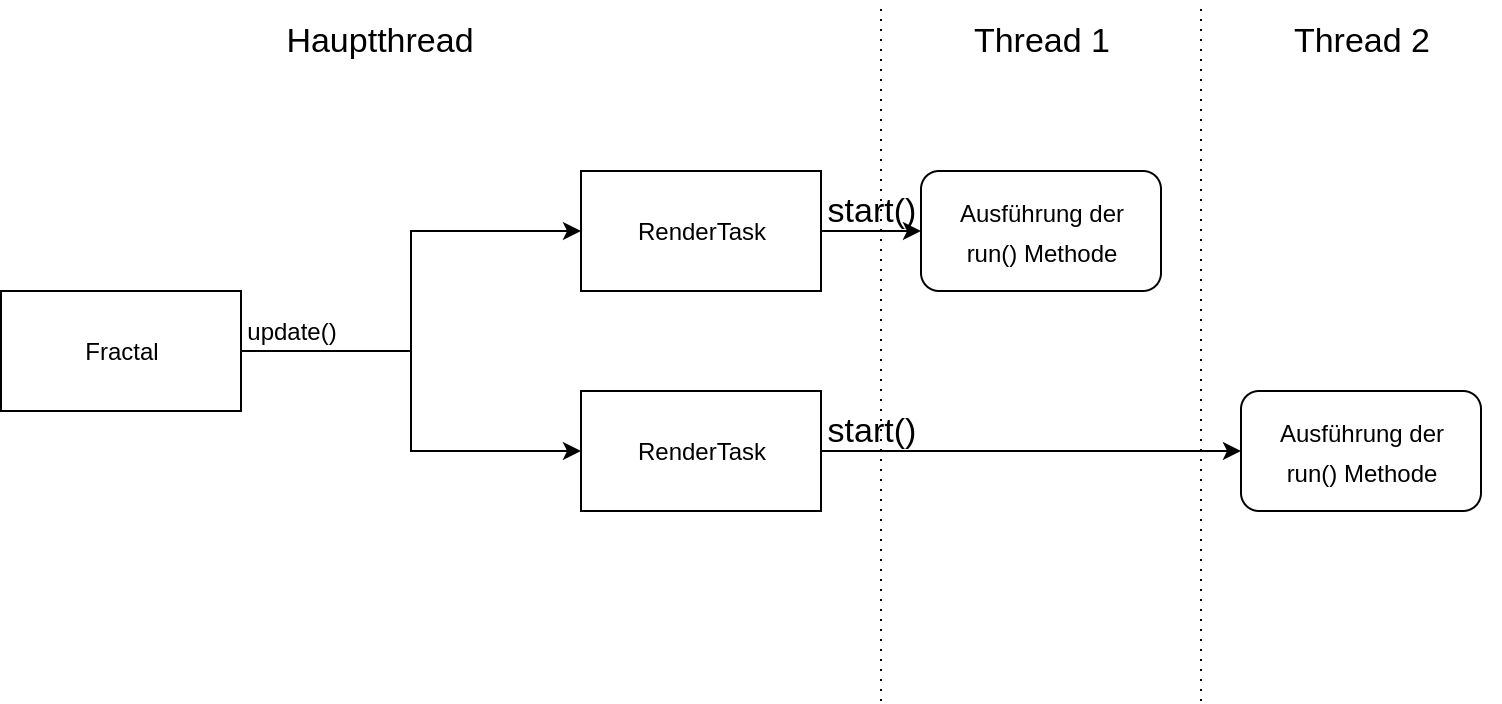
\includegraphics[width=1.0\textwidth]{images/thread-diagram.png}
  \begin{itemize}
    \item QThread ist eine Verwaltungs-Klasse eines Threads
    \item Startet einen Thread mit der Funktion \emph{QThread::start()}
  \end{itemize}
\end{frame}

\begin{frame}
  \frametitle{QThread}
  \begin{figure}
    \centering
    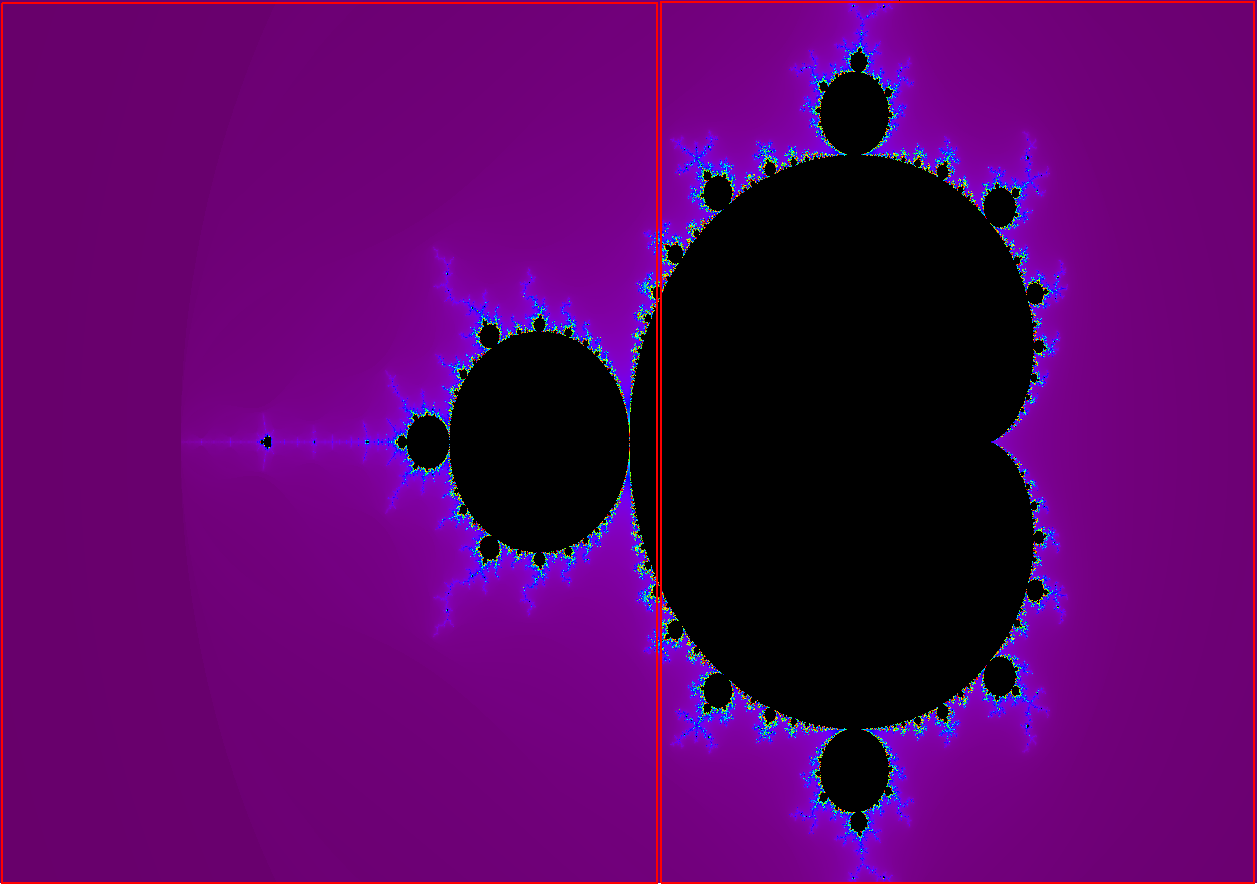
\includegraphics[width=0.8\textwidth]{images/fractal-mandelbrot-threads.png}
  \end{figure}
\end{frame}

\subsection{Optimierungen bei der Berechnung}
\begin{frame}
  \frametitle{Mandelbrot- \& Julia-Menge}
  \begin{itemize}
    \item Ignorieren der schwarzen Flächen
    \item Interpolation zwischen zwei Pixeln
  \end{itemize}
\end{frame}
\begin{frame}
  \frametitle{Kochkurve}
  \begin{itemize}
    \item Einführen von Clipping
    \item Abbrechen der Berechnung, wenn Linie kleiner als 1px
  \end{itemize}
\end{frame}


\end{document}
